%%%%%%%%%%%%%%%%%%%%%%%%%%%%%%%%%%%%%%%%%%%%%%%%%%%%%%%%%%%%
\documentclass[xcolor=x11names,compress]{beamer}
%\documentclass[handout]{beamer}
\definecolor{CoolBlack}{rgb}{0.0, 0.18, 0.39}
\definecolor{byellow}{rgb}{0.55037, 0.38821, 0.06142}
%% General document %%%%%%%%%%%%%%%%%%%%%%%%%%%%%%%%%%
\usepackage{graphicx}
\usepackage{tikz}
\usepackage{Tabbing, tabu}
\usetikzlibrary{decorations.fractals}
%%%%%%%%%%%%%%%%%%%%%%%%%%%%%%%%%%%%%%%%%%%%%%%%%%%%%%

%% Beamer Layout %%%%%%%%%%%%%%%%%%%%%%%%%%%%%%%%%%
\useoutertheme[subsection=false,shadow]{miniframes}
\useinnertheme{default}
\usefonttheme{serif}
\usepackage{palatino}
\usepackage{tabu}

\usepackage{subfigure}

% addition of color
\usepackage{xcolor}
\definecolor{dgreen}{rgb}{0.,0.6,0.}
\definecolor{RawSienna}{cmyk}{0,0.72,1,0.45}

\setbeamerfont{title like}{shape=\scshape}
\setbeamerfont{frametitle}{shape=\scshape}

\setbeamercolor*{lower separation line head}{bg=CoolBlack} 
\setbeamercolor*{normal text}{fg=black,bg=white} 
\setbeamercolor*{alerted text}{fg=dgreen} 
\setbeamercolor*{example text}{fg=black} 
\setbeamercolor*{structure}{fg=black} 
 
\setbeamercolor*{palette tertiary}{fg=black,bg=black!10} 
\setbeamercolor*{palette quaternary}{fg=black,bg=black!10} 

% Links
\usepackage{hyperref}
\definecolor{links}{HTML}{003262}
\hypersetup{colorlinks,linkcolor=,urlcolor=links}

% columns
\renewcommand{\(}{\begin{columns}}
\renewcommand{\)}{\end{columns}}
\newcommand{\<}[1]{\begin{column}{#1}}
\renewcommand{\>}{\end{column}}

% adding slide numbers
\addtobeamertemplate{navigation symbols}{}{%
    \usebeamerfont{footline}%
    \usebeamercolor[fg]{footline}%
    \hspace{1em}%
    \insertframenumber/\inserttotalframenumber
}

% equation stuff
\newcommand{\Macro}{\ensuremath{\Sigma}}
\newcommand{\Sn}{\ensuremath{S_N} }
\newcommand{\vOmega}{\ensuremath{\hat{\Omega}}}
\usepackage{mathrsfs}
\usepackage[mathcal]{euscript}
\usepackage{amssymb}
\usepackage{amsthm}
\usepackage{epsfig}
\usepackage{amsmath}

\newcommand{\ve}[1]{\ensuremath{\vec{#1}}}
\newcommand{\micro}{\ensuremath{\sigma}}
\newcommand{\detR}{\ensuremath{\Sigma}}

\newcommand{\vecr}{\vec{r}}
\newcommand{\sn}{S$_\mathrm{N}$~}
\newcommand{\pn}{P$_\mathrm{N}$~}
\newcommand{\sigt}{\Sigma_t}
\newcommand{\sigs}{\Sigma_s}
\newcommand{\hn}{\mathcal{H}_N}
\newcommand{\maths}{\mathbb{S}^2}
\newcommand{\dn}{d_N}
\newcommand{\lij}{\langle L_i,L_j \rangle}

\newcommand{\Jij}[2]{\ensuremath{\int L(\vOmega_#1)L(\vOmega_#2)}}
\newcommand{\Gij}[2]{\ensuremath{\sum_{\ell=0}^L \frac{2\ell +1}{4\pi}P_{\ell}(\vOmega_#1 \cdot\vOmega_#2)}}
\newcommand{\LijJij}[4]{\ensuremath{\int L_#1(\vOmega_#3)L_#2(\vOmega_#4)}}
\newcommand{\Sij}[2]{\ensuremath{\Sigma^{g'\rightarrow g}_{\text{s,N}}(\vOmega_#1 \cdot \vOmega_#2)}}

\newcommand{\sigg}[1]{\ensuremath{\sigma^{gg'}_{\text{s}\,#1}}}
\newcommand{\Sigg}[1]{\ensuremath{\Sigma^{gg'}_{\text{s}\,#1}}}
\newcommand{\psig}{\ensuremath{\psi^g}}
\newcommand{\ldosig}[2]{\ensuremath{\sum_{n=0}^N \frac{2n+1}{4\pi}\sigma_{s,n}^{g'\rightarrow g} P_n(\vOmega_#1\cdot\vOmega_#2)}}

% Define plus minus symbol
\makeatletter
\newcommand{\mypm}{\mathbin{\mathpalette\@mypm\relax}}
\newcommand{\@mypm}[2]{\ooalign{%
  \raisebox{.1\height}{$#1+$}\cr
  \smash{\raisebox{-.6\height}{$#1-$}}\cr}}
\makeatother

% Math packages
\newenvironment{myalign}{\par\nobreak\small\noindent\align}{\endalign}
\usepackage[version=3]{mhchem}
\usepackage{esint}
\usepackage{esvect}
\usepackage{siunitx}
\usepackage{mathtools}
\DeclarePairedDelimiter\abs{\lvert}{\rvert}%

\newcommand\RBox[1]{%
  \tikz\node[draw,rounded corners,align=center,] {#1};}%

\setbeamerfont{author in head/foot}{size={\fontsize{3pt}{4pt}\selectfont}}
%\author[Subham \& Mithun \& Karthikeyan \& Shantikumar]
%{%
%   \texorpdfstring{
%        \begin{columns}
%            \column{.25\linewidth}
%            \centering
%            \includegraphics[height=3cm]{../bk-eps-converted-to}
%            \column{.25\linewidth}
%            \centering
%            \RBox{R.\ N.\ Slaybaugh\\
%            Univ.\ of Cal.\ Berkeley}\\[1ex]
%            \RBox{T.\ M.\ Evans, and\\
%            S.\ W.\ Mosher\\
%            Oak Ridge National Lab}
%        \end{columns}
%   }
%   {Subham Soni S., Karthikeyanm, Shantikumar L.,  Mithun C.K.}
%}
\title{Advanced Solvers and Challenges for Nuclear Innovation}
\author{\includegraphics[height=2cm]
{../bk-eps-converted-to}\\R.\ N.\ Slaybaugh, Univ.\ of Cal.\ Berkeley
}
\date{12 May 2017 \\ IBT Seminar, LBNL}

%%%%%%%%%%%%%%%%%%%%%%%%%%%%%%%%%%%%%%%%%%%%%%%%%%

\begin{document}

%%%%%%%%%%%%%%%%%%%%%%%%%%%%%%%%%%%%%%%%%%%%%%%%%%%%%%
%%%%%%%%%%%%%%%%%%%%%%%%%%%%%%%%%%%%%%%%%%%%%%%%%%%%%%
\begin{frame}
\titlepage
\end{frame}

% --------------------------------------------------------------
\begin{frame}[fragile]{Outline}
  \frametitle{Nuclear innovation is needed}

\begin{columns}
  \begin{column}{0.5\textwidth}
  		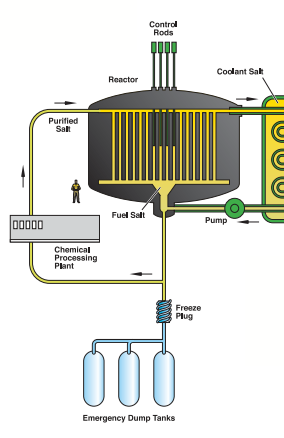
\includegraphics[height=2.75in,clip]{../figs/msr-core-diagram}
		%\caption{advanced reactors}
  \end{column}
  \begin{column}{0.5\textwidth}
        \renewcommand*{\thesubfigure}{}
      \begin{figure}[htp]
        \centering
        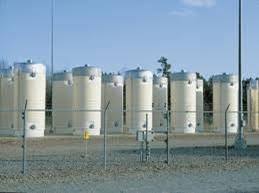
\includegraphics[width=1.75in]{../figs/isfsi}

        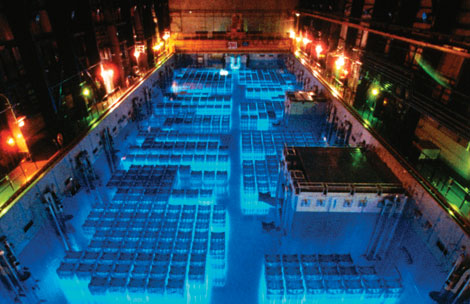
\includegraphics[width=1.75in]{../figs/spent-fuel-pool}
      \end{figure}    
  \end{column}
\end{columns}

\end{frame}

% --------------------------------------------------------------
\begin{frame}[fragile]{Outline}
  \frametitle{Outline}

\begin{columns}
  \begin{column}{0.5\textwidth}
    \begin{itemize}
    \item Motivation \& Background
    \vspace*{.5em}
    \item Hybrid Methods and Strong Anisotropies
        \begin{itemize}
        \item Research Objectives
	\item CADIS-$\Omega$ Method
	\item LDO Method
        \end{itemize}
        
   \vspace*{.5em}
   \item Spectrum Shaping for Strategic Research
        \begin{itemize}
        \item Research Objectives
	\item Gnowee: Metaheuristic Optimization Algorithm
	\item Coeus: ETA Design Software
        \end{itemize}	
  \end{itemize}
  \end{column}
  \begin{column}{0.5\textwidth}
  	\begin{figure}
  	\begin{center}
  		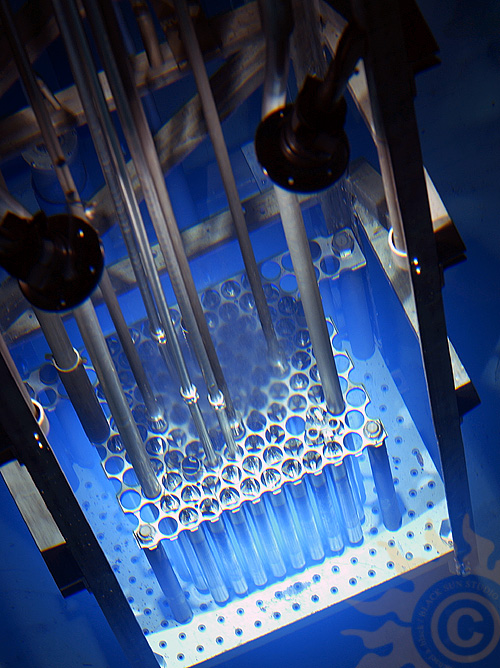
\includegraphics[height=2.5in,clip]{../figs/psu-reactor}
	\end{center}
  	\end{figure}
  \end{column}
\end{columns}

\end{frame}


% --------------------------------------------------------------
% --------------------------------------------------------------
\section{\scshape Motivation \& Background}
\begin{frame}[fragile]
  \frametitle{Numerical methods for radiation transport}

\begin{columns}
  \begin{column}{0.55\textwidth}
  To facilitate nuclear innovation, 
we need predictive simulation
	\begin{itemize}
	\item I build tools (translate applied math into code) used to design and analyze nuclear systems
	\item I focus on high performance computing
	\item and inform algorithm development with physics of problems of interest
	\end{itemize}
  \end{column}
  \begin{column}{0.45\textwidth}
  	\begin{figure}
  	\begin{center}
  		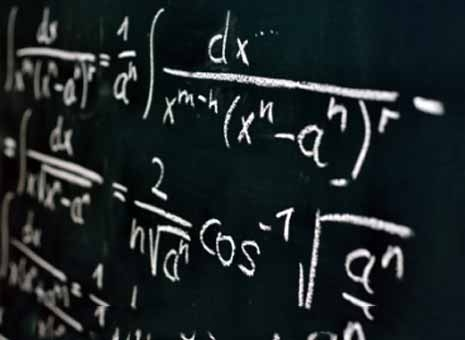
\includegraphics[height=1.in,clip]{../figs/applied-math}\\
		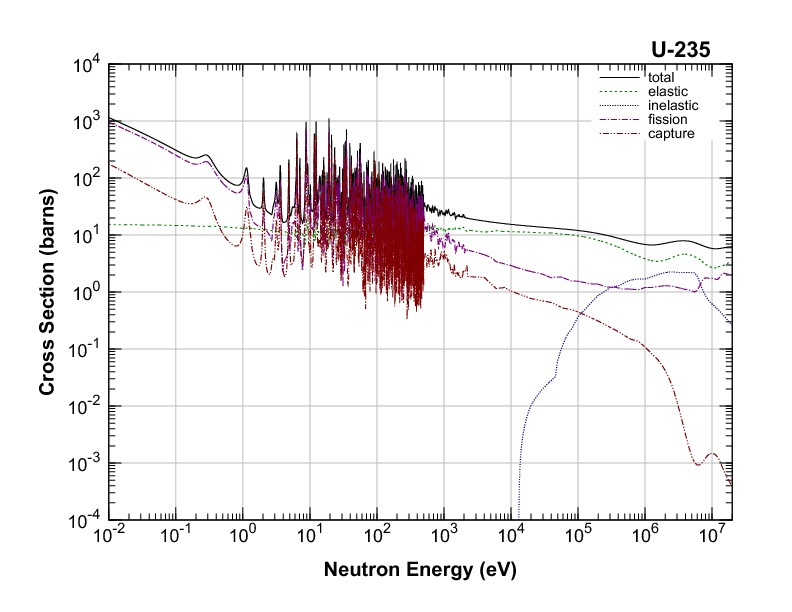
\includegraphics[height=1.5in,clip]{../figs/u235-xsecs}
	\end{center}
  	\end{figure}
  \end{column}
\end{columns}

\end{frame}


% --------------------------------------------------------------
% --------------------------------------------------------------
\begin{frame}[fragile]
  \frametitle{Solving the TE}
  %
  \begin{align}
\vOmega \cdot \nabla \psi(\vec{r}, E, \vOmega) &+
\Sigma_t \psi(\vec{r}, E, \vOmega) = S(\vec{r}, E, \vOmega) \:+\nonumber\\
%
& \int_{4\pi} d\vOmega' \int_0^{\infty} dE'\: \Sigma_s(E', \vOmega' \rightarrow E, \vOmega) \psi(\vec{r}, E', \vOmega') \nonumber
\end{align}
%
\begin{columns}
  \begin{column}{0.5\textwidth}
  \begin{center}
  \underline{Monte Carlo}
  \end{center}
  \vspace*{-1em}
	\begin{itemize}
	\item \textit{Continuous} phase space%: ``gold standard answers"
	\item Solution has statistical error
	\item Localized solutions
	\item Optically thick = \textit{slow}
	\end{itemize}
  \end{column}
  \begin{column}{0.5\textwidth}
  \begin{center}
  \underline{Deterministic}
  \end{center}
  \vspace*{-1em}
	\begin{itemize}
	\item \textit{Discretized} phase space%: drives solution quality
	\item Solution equally valid everywhere
	\item Truncation errors
	\item Streaming = \textit{ray effects}
	\end{itemize}
  \end{column}
\end{columns}

\end{frame}

% --------------------------------------------------------------
\begin{frame}[fragile]
  \frametitle{Speeding up MC}
  \begin{itemize}
	\item Variance reduction (VR) used to improve Monte Carlo:\\
	reduce relative error \textit{and} time by augmenting game
	\item Particles are assigned weights that map to impact
	\item VR can be used to
	  \begin{itemize}
	  \item set weights at birth
	  \item update weights throughout problem
      \end{itemize}
      \pause
  \item Improvement measured as    
  \end{itemize}
\[
\text{FOM} = \frac{1}{\text{R}^2\text{t}} \quad \text{R = relative error;  t = time} 
\]
\pause
\textbf{Hybrid Methods:} we use deterministic results to make Monte Carlo VR parameters

\end{frame}


% --------------------------------------------------------------
% --------------------------------------------------------------
\section{\scshape Hybrid Methods \& Anisotropy}

\begin{frame}[fragile]
  \frametitle{Project 1 motivation}
%
%\begin{columns}
%  \begin{column}{0.55\textwidth}
%	\begin{itemize}
%	\item Need to accurately model radiation for safeguarding and monitoring
%	\item \alert{Challenging}: dense shields; streaming paths
%	\item Current methods are insufficient
%	\item \alert{Goal}: accurate solutions in reasonable time
%	\item New methods can easily be added to existing codes
%	\end{itemize}
%  \end{column}
%  \begin{column}{0.45\textwidth}
%  	\begin{figure}
%  	\begin{center}
%  		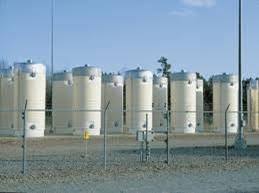
\includegraphics[height=1.5in,clip]{../figs/isfsi}
%		\caption{Used fuel storage pad}
%	\end{center}
%  	\end{figure}
%  \end{column}
%\end{columns}
%
%\end{frame}
%
%
%% --------------------------------------------------------------
%% --------------------------------------------------------------
%\begin{frame}[fragile]
%  \frametitle{Anisotropy: a computational challenge}

	\begin{columns}
  	\begin{column}{0.5\textwidth}
	\begin{itemize}
	\item Many important nuclear applications have strong anisotropies
	 \begin{itemize}
	 \item \textbf{Used fuel casks}
	 \item \textbf{Reprocessing facilities}
	 \item Reactor facilities
	 \item Active interrogation 
	 \end{itemize}
	\pause
	\item New ideas are needed for these problems
	\begin{itemize}
	\item Current hybrid methods are only $f(\vec{x}, E)$
	\item Including angle explicitly is too costly	
	\end{itemize}
	\pause
	\item \alert{Goal}: new methods that are easy to use
	\end{itemize}
  	\end{column}
 	%
 	\begin{column}{0.5\textwidth}
 	 \begin{center}
 	 \begin{figure}
 	 \includegraphics[height=2in,clip]{../figs/pwr}  
 	 \caption{PWR relative error \cite{Pantelias2013}}
 	 \end{figure}
 	 \end{center}

  	\end{column}
	\end{columns}

\end{frame}



%% --------------------------------------------------------------
%\begin{frame}[fragile]
%  \frametitle{Forward-Adjoint Relationship \cite{Wagner2007}}
%Define response with function $f(\ve{r}, E)$ in volume $V_f$ as
%%
%\begin{equation}
% R = \int_E \int_{V_f} f(\ve{r}, E) \phi(\ve{r}, E) dV dE 
% \label{eq:Response}
%\end{equation}
%%
%\begin{columns}
%  \begin{column}{0.5\textwidth}
%	\begin{align}
%  	H\phi &= q \quad \text{(forward)}\nonumber \\
%  	%
%  	H^{\dagger} \phi^{\dagger} &= q^{\dagger} \quad 
%  	\text{(adjoint)}\nonumber
%  	\end{align}
%  \end{column}
%  \begin{column}{0.5\textwidth}
%  	\begin{align}
%  	\langle H\phi, \phi^{\dagger} \rangle &= \langle H^{\dagger} \phi^{\dagger}, \phi \rangle \:, \text{and therefore} \nonumber \\
%  	%
%  	\langle q, \phi^{\dagger} \rangle &= \langle q^{\dagger}, \phi \rangle \nonumber
%  	\end{align}
%  \end{column}
%\end{columns}
%\vspace*{1 em}
%If we let $q^{\dagger} = f(\ve{r}, E)$ then
%%
%\begin{equation}
% \langle q^{\dagger}, \phi \rangle = \langle f, \phi \rangle = R = \langle q, \phi^{\dagger} \rangle
% \label{eq:ResponseRedef}
%\end{equation}
%%
%Eq.\ \eqref{eq:ResponseRedef} expresses that $\phi^{\dagger}$ represents the expected contribution of a source particle to the response given the source, $q$.
%
%\end{frame}
%
%% --------------------------------------------------------------
%\begin{frame}[fragile]
%  \frametitle{CADIS \cite{Wagner2007}}
%  
%  \begin{enumerate}
%  \item Define $q^{\dagger}$ as the local response of interest\\
%  \item Coarse deterministic calculation to get $\phi^{\dagger}$ and $R$
%  \end{enumerate}
%% 
%\begin{align}
%  imp(\ve{r}, E) &= \frac{\phi^{\dagger}(\ve{r}, E)}{\langle q(\ve{r}, E), \phi^{\dagger}(\ve{r}, E) \rangle} = \frac{\phi^{\dagger}(\ve{r}, E)}{R} \\
%  %
%  \hat{q}(\ve{r}, E) &= \frac{\phi^{\dagger}(\ve{r}, E) q(\ve{r}, E)}{R} \\
%  %
%  w_0(\ve{r}, E) &= \frac{q(\ve{r}, E)}{\hat{q}(\ve{r}, E)} = \frac{R}{\phi^{\dagger}(\ve{r}, E)} 
%  \label{eq:Importance}
%\end{align}
%
%Birth weights match weight targets, making this the \underline{C}onsistent \underline{A}djoint \underline{D}riven \underline{I}mportance \underline{S}ampling \underline{M}ethod
%
%\end{frame}
%
%% --------------------------------------------------------------
%%\subsection{FW-CADIS}
%\begin{frame}[fragile]
%  \frametitle{FW-CADIS \cite{Wagner2007}}
%
%\begin{itemize}
%\item We often what to optimize solutions in all of phase space\\
%\item In this case the adjoint source needs to be a global forward solution: \underline{F}orward \underline{W}eighted-CADIS
%\end{itemize}
%%
%\begin{columns}
%  \begin{column}{0.5\textwidth}
%  \begin{center}
%  \alert{To Optimize}
%  \end{center}
%	\begin{align}
%  	&\phi(\ve{r}, E)\nonumber \\
%  	%
%  	\int&\phi(\ve{r}, E)\sigma_d(\ve{r}, E)\nonumber
%  	\end{align}
%  \end{column}
%  %
%  \begin{column}{0.5\textwidth}
%  \begin{center}
%  \alert{Adjoint Source}
%  \end{center}
%  	\begin{align}
%  	f(\ve{r}, E) &= \frac{1}{\phi(\ve{r}, E)}\nonumber \\
%  	%
%  	f(\ve{r}, E) &= \frac{\sigma_d(\ve{r}, E)}{\int\phi(\ve{r}, E)\sigma_d(\ve{r}, E)} \nonumber
%  	\end{align}
%  \end{column}
%\end{columns}
%\vspace*{1 em}
%For example
%%
%\begin{equation}
% R = \int_E \int_{V_f} f(\ve{r}, E) \phi(\ve{r}, E) dV dE = \int_E \int_{V} \frac{1}{\phi(\ve{r}, E)} \phi(\ve{r}, E) dV dE \approx 1 \nonumber
%\end{equation}
%
%\end{frame}


% --------------------------------------------------------------
\begin{frame}[fragile]
  \frametitle{Adjoint as an importance map}
Define response with function $f(\ve{r}, E)$ in volume $V_f$ as
%
\begin{equation}
 R = \int_E \int_{V_f} f(\ve{r}, E) \phi(\ve{r}, E) dV dE 
 \label{eq:Response}
\end{equation}
\pause
\begin{itemize}
\item Forward ($\phi$ or $\psi$): neutrons flow from the source ($q$) to the detector
\item Adjoint($\phi^{\dagger}$ or $\psi^{\dagger}$): particles represent how each part of phase space contributes to the ``source" ($q^{\dagger}$)
\item $\phi^{\dagger}$ represents the expected contribution of a source particle to the response given the source, $q$.
\end{itemize}


\end{frame}
% --------------------------------------------------------------
% --------------------------------------------------------------
\begin{frame}[fragile]

  \frametitle{Understanding Forward flux}
  10 MeV isotropic point source; NaI detector
  \begin{columns}
   \begin{column}{0.75\textwidth}
   \begin{figure}
   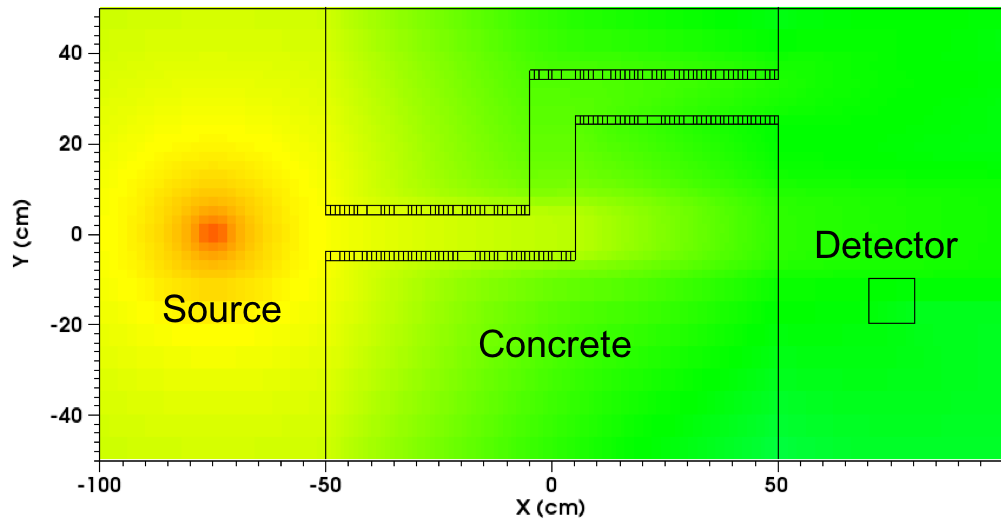
\includegraphics[height=1.5in,clip]{../figs/maze-forward.png}
   %\caption{Simple two-turn labyrinth}
   \end{figure}
   \end{column}
  %
  \begin{column}{0.25\textwidth}
Neutrons in the forward problem will flow from the source to the detector
   \end{column}
\end{columns}
	
\end{frame}

%% --------------------------------------------------------------
%
\begin{frame}[fragile]
  \frametitle{Understanding Adjoint Flux}
  10 MeV isotropic point source; NaI detector
  \begin{columns}
   \begin{column}{0.25\textwidth}
   Adjoint measures how each part of phase space contributes to the solution: \\
\vspace*{.5em}
\alert{importance map} 
   \end{column}
  %
  \begin{column}{0.75\textwidth}
   \begin{figure}
   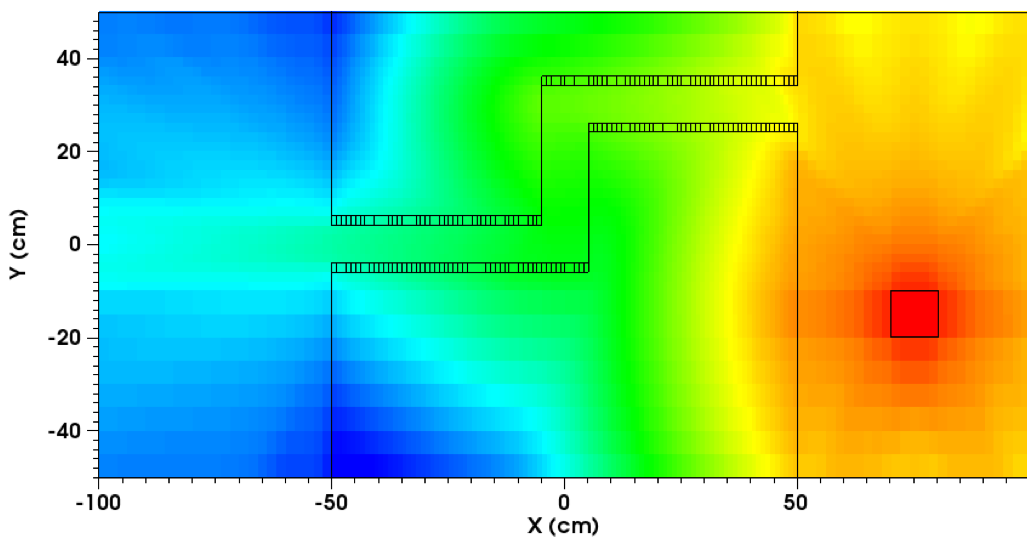
\includegraphics[height=1.75in,clip]{../figs/maze-adjoint.png}
   %\caption{Simple two-turn labyrinth}
   \end{figure}
   \end{column}
\end{columns}
\end{frame}


% --------------------------------------------------------------
\begin{frame}[fragile]
  \frametitle{Adjoint as an importance map}
Use \textit{adjoint}: the importance of a source particle to the solution

\begin{itemize}
\item Define $q^{\dagger}$ as the response of interest
\item Coarse deterministic calculation to get $\phi^{\dagger}$ and $R$
\item The current state of the art is FW/CADIS \cite{Wagner2007}
\end{itemize}
\begin{align*}
  imp(\ve{r}, E) &= \frac{\phi^{\dagger}(\ve{r}, E)}{\langle q(\ve{r}, E), \phi^{\dagger}(\ve{r}, E) \rangle} = \frac{\phi^{\dagger}(\ve{r}, E)}{R} \\
  %
  \hat{q}(\ve{r}, E) &= \frac{\phi^{\dagger}(\ve{r}, E) q(\ve{r}, E)}{R} \\
  %
  w_0(\ve{r}, E) &= \frac{q(\ve{r}, E)}{\hat{q}(\ve{r}, E)} = \frac{R}{\phi^{\dagger}(\ve{r}, E)} 
\end{align*}

\end{frame}


% --------------------------------------------------------------
\begin{frame}[fragile]
  \frametitle{Current hybrid methods are insufficient}

\[\text{Note:}\qquad\phi^{\dagger}(\ve{r},E) = \int \psi^{\dagger}(\vOmega, 
		\ve{r},E) d\vOmega\]

	\begin{itemize}
	\item MC VR parameters created from adjoint deterministic scalar flux that is a function of \textit{space and energy only} \vspace*{1 em}
	\pause
	\item Angular dependence of the importance function is not retained, otherwise the map would be 
	\begin{itemize}
	  \item very large (tens or hundreds of GB) and
	  \item more costly and complex to use in the MC simulation 
	\end{itemize}
	\pause
	\item Drawback: within a given space/energy cell, map provides average importance of a particle moving in \textit{any direction} through the cell--excluding information about how particles move \alert{toward the objective}
	\end{itemize}

\end{frame}

% --------------------------------------------------------------
\begin{frame}[fragile]
  \frametitle{Current hybrid methods are insufficient}

	\begin{columns}
  	\begin{column}{0.5\textwidth}
 	 \begin{center}
 	 \begin{figure}
 	 \includegraphics[height=2in,clip]{../figs/boat-interrogation}  
 	 \caption{Spherical boat model with source on left and fissionable material at center}
 	 \end{figure}
 	 \end{center}
  	\end{column}
 	%
 	\begin{column}{0.5\textwidth}
 	 \begin{center}
 	 \begin{figure}
 	 \includegraphics[height=2in,clip]{../figs/boat-map}  
 	 \caption{Target weight window values for 14.1 MeV neutrons}
 	 \end{figure}
 	 \end{center}
  	\end{column}
	\end{columns}

\end{frame}

% --------------------------------------------------------------
% --------------------------------------------------------------
% --------------------------------------------------------------
\begin{frame}[fragile]
  \frametitle{Integration weighting}

    Different integration plan captures angles in scalar flux creation	
	\begin{align*}
		\phi^{\dagger}(\ve{r},E) &= \int \psi^{\dagger}(\vOmega, 
		\ve{r},E) d\vOmega \qquad  \qquad \qquad \text{original}\\
		 %
		\phi^{\dagger}(\ve{r},E) &= \frac{\int \psi(\vOmega, \ve{r},E)
		 \psi^{\dagger}(\vOmega, \ve{r},E) d\vOmega}{\int \psi(\vOmega, 
		 \ve{r},E)  d\vOmega} \qquad \text{\alert{new}}
	\end{align*}
%Note that these two calculations can be completed concurrently. Then, the adjoint scalar fluxes will be computed by angularly integrating the product of the forward and adjoint angular fluxes to account for the directions in which the particles will actually be traveling at any given location/energy:
%will provide importance values that more accurately reflect the average importance of particles that will be transported in the final Monte Carlo calculation, yielding faster Monte Carlo run times.
    \pause
    Major challenges and areas of investigation:
	\begin{enumerate}
	\item Data storage and handling (many GBs)
	\item More, less, or differently sensitive to 
	  \begin{itemize}
	  \item quality of the discrete ordinates calculation?
	  \item ray effects?
	  \end{itemize}
	\end{enumerate}

\end{frame}


% --------------------------------------------------------------
\begin{frame}[fragile]
  \frametitle{Method implementation}

  	\begin{itemize}
    \item The space- and energy-dependent importance map is normalized and 
     source biasing parameters are generated in the \alert{same ways} as
     the current implementation of FW/CADIS \vspace*{1 em}
	\item Immediately useful; widely applicable \vspace*{1 em}
	\item We are studying and characterizing the impact\vspace*{1 em}
	\item Is available ADVANTG \cite{mosher_new_2010}
	\end{itemize}
	
\end{frame}


% --------------------------------------------------------------
% --------------------------------------------------------------
%\section{\scshape Results \& Plans}
%\begin{frame}[fragile]
%  \frametitle{Current Status}
%
%    \begin{enumerate}
%    \item Implementation: \alert{complete}
%      \begin{itemize}
%      %\item Large data handling is \alert{broader outcome}
%      \item Implementation of weighted flux algorithm in Denovo \cite{Evans2010} is 
%      complete
%      \item Integration of method into ADVANTG complete
%      %\item ADVANTG allows for ease of use; broader user base
%      %\item Denovo integration enhances use on other hybrid platforms
%      \end{itemize} 
%      \vspace*{0.5em}
%      \pause
%    \item Testing: \alert{in process}
%      \begin{itemize}
%      \item A collection of small tests with varying anisotropies
%      \item Studying performance compared to existing methods as a function of degree of anisotropy
%      \item Investigating impact of angular discretization
%      \end{itemize}
%      \vspace*{0.5em}
%      \pause
%    \item Impact characterization: \alert{started}
%      \begin{itemize}
%      \item Investigating performance for one used fuel canister
%      \item Investigating performance for array of used fuel canisters
%      \item Extending to other applications of interest like monitoring reprocessing
%      \end{itemize}
%    \end{enumerate}
%
%	
%\end{frame}


%% --------------------------------------------------------------
\begin{frame}[fragile]
  \frametitle{The New Method Captures Anisotropy}
Comparing the original adjoint to CADIS-$\Omega$....
  \begin{columns}
    \begin{column}{0.5\textwidth}
  	\begin{figure}
  	\begin{center}
  		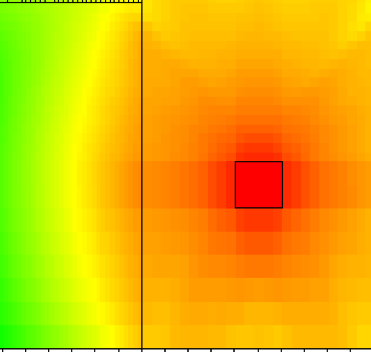
\includegraphics[height=1.1in,clip]{../figs/maze-adj-orig.png}
		\caption{original adjoint}
	\end{center}
  	\end{figure}
    \end{column}
  \pause
    \begin{column}{0.5\textwidth}
     	  \begin{figure}
  	\begin{center}
  		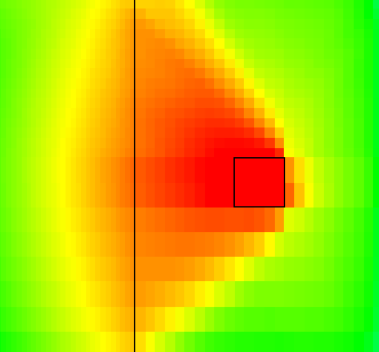
\includegraphics[height=1.1in,clip]{../figs/maze-adj-new}
		\caption{new adjoint}
		% point out that while the FOM is better for analog, it has high RE in regions, so overall it performs poorer
	\end{center}
  	\end{figure}
  	\end{column}  
  \end{columns}
  ...shows that the method does incorporate problem physics differently
\end{frame}

%% --------------------------------------------------------------
%
\begin{frame}[fragile]
  \frametitle{Response in Maze Detector}
  
\begin{columns}
  \begin{column}{0.45\textwidth}
  CADIS-$\Omega$ has:
  \begin{itemize}
    \item Relatively uniform uncertainty distribution
    \item Faster runtimes than CADIS
  \end{itemize}
  \vspace*{.5em}
  \begin{tabular}{|l|c c|}
  \hline
      Run Type & Time (m) & FOM \\  
      \hline
      CADIS  & 524.9  &  5.1 \\
      CADIS-$\Omega$ & 491.9 & 145 \\
      \hline
  \end{tabular}
  \end{column}
  \begin{column}{0.55\textwidth}
  	\begin{figure}
  	\begin{center}
  		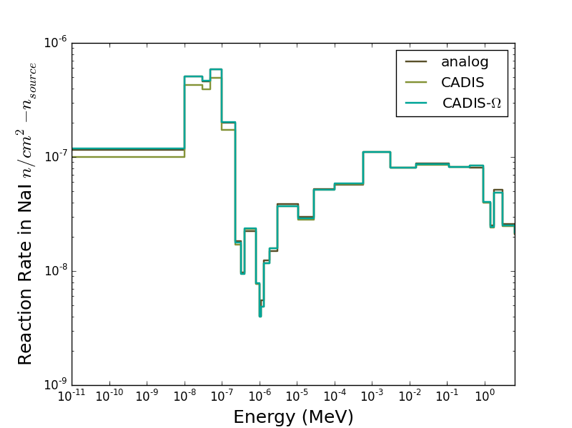
\includegraphics[height=1.5in,clip]{../figs/maze-results.png}\\
		%\caption{Response for maze 2}
  		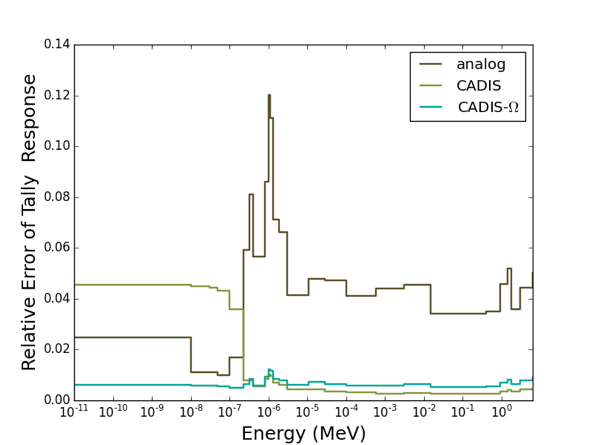
\includegraphics[height=1.5in,clip]{../figs/maze-re.png}
		%\caption{Relative errors for response function}
		% point out that while the FOM is better for analog, it has high RE in regions, so overall it performs poorer
	\end{center}
  	\end{figure}
  \end{column}
\end{columns}
\end{frame}



%% --------------------------------------------------------------
\begin{frame}[fragile]

  \frametitle{Quantifying Anisotropy}
  
  To measure how the method performs based on the degree of problem anisotropy, we've defined several metrics
  \vspace*{1em}
    \begin{columns}
    \begin{column}{0.5\textwidth}
      \begin{itemize}
      \item $M_{1} = \frac{\phi^{\dagger}(\vecr,E)\phi(\vecr,E)}{\int_{\vOmega}\psi^{\dagger}(\vecr,\vOmega,E)\psi(\vecr,\vOmega,E)}$
      \item $M_{2} = \frac{\phi^{\dagger}_{\vOmega}(\vecr,E)}{\phi^{\dagger}(\vecr,E)}$
      \item $M_{3} = \frac{\max(\int_{\vOmega}\psi^{\dagger}(\vecr,\vOmega,E)\psi(\vecr,\vOmega,E))}{\text{avg}(\int_{\vOmega}\psi^{\dagger}(\vecr,\vOmega,E)\psi(\vecr,\vOmega,E))}$
       \item $M_{4} = \frac{\max(\int_{\vOmega}\psi^{\dagger}(\vecr,\vOmega,E)\psi(\vecr,\vOmega,E))}{\min(\int_{\vOmega}\psi^{\dagger}(\vecr,\vOmega,E)\psi(\vecr,\vOmega,E))}$
      \end{itemize}
    \end{column}    
    \begin{column}{0.5\textwidth}
    Example: source in a room
      	\begin{figure}
  	\begin{center}
  		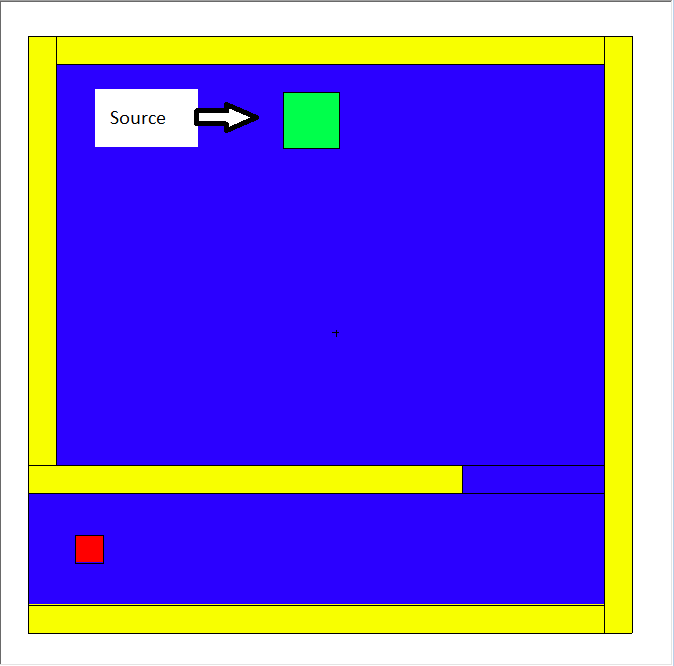
\includegraphics[height=1.5in,clip]{../figs/therapy-room.png}
	\end{center}
  	\end{figure}
    \end{column}
  \end{columns}   

\end{frame}


%% --------------------------------------------------------------
\begin{frame}[fragile]
  \frametitle{Response in Room Detector}
  
\begin{columns}
  \begin{column}{0.45\textwidth}
  CADIS-$\Omega$ again has:
  \begin{itemize}
    \item Relatively uniform uncertainty distribution
    \item Faster runtimes than CADIS
  \end{itemize}
  \vspace*{.5em}
  \begin{tabular}{|l|c c|}
  \hline
      Run Type & Time (m) & FOM \\  
      \hline
      CADIS  & 69.05  &  287 \\
      CADIS-$\Omega$ & 50.4 & 373 \\
      \hline
  \end{tabular}
  \end{column}
  \begin{column}{0.55\textwidth}
  	\begin{figure}
  	\begin{center}
  		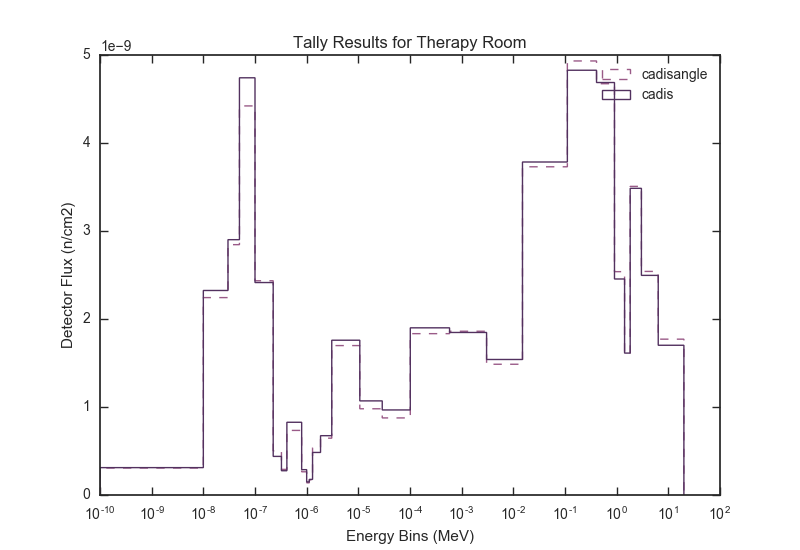
\includegraphics[height=1.5in,clip]{../figs/room-both-tally.png}\\
		%\caption{Response for maze 2}
  		\includegraphics[height=1.5in,clip]{../figs/room-both-re.png}
		%\caption{Relative errors for response function}
		% point out that while the FOM is better for analog, it has high RE in regions, so overall it performs poorer
	\end{center}
  	\end{figure}
  \end{column}
\end{columns}
\end{frame}


%% --------------------------------------------------------------
\begin{frame}[fragile]

  \frametitle{Impact Tests}
  
    \begin{columns}
    \begin{column}{0.55\textwidth}
    Real system tests will show the ability of the method to improve MC for applications of interest\\
    \vspace*{1em}
    We are starting with a full storage cask with highly-detailed information
    \end{column}    
    \begin{column}{0.45\textwidth}
  \begin{center}
  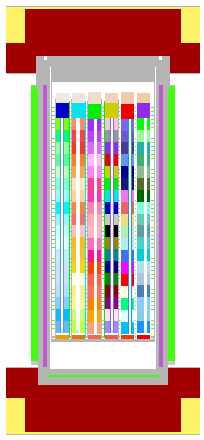
\includegraphics[height=2.5in,clip]{../figs/Transfer_Side_profile}  
  \end{center}
    \end{column}
  \end{columns}   

\end{frame}

% --------------------------------------------------------------
% --------------------------------------------------------------


%% --------------------------------------------------------------
%% --------------------------------------------------------------
%\section{\scshape LDO Method}
\begin{frame}[fragile]

  \frametitle{Lagrange Discrete Ordinates (LDO) \cite{Ahrens2015}}

   We're also looking at an entirely different approach.    
\pause
\begin{itemize}
\item{Formally the same as the classical $S_N$ equations}
	\begin{itemize}
	\pause
	\item{The difference lies in how the scattering source is calculated and in the representation of the angular flux}
	\pause
	\item{\textbf{No need to evaluate spherical harmonic moments of angular flux}}
	\end{itemize}
\pause
\item{Increasing the angular resolution of the LDO equations brings ability to mitigate ray effects}
%	\begin{itemize}
%	\pause
%	\item{Positive-weight quadrature sets on which LDO equations are based can integrate spherical harmonics from degree 0 to degree 165}
%	\pause
%	\item{For a fixed maximum degree of integration $N$, the corresponding number of quadrature points (ordinates) is $(N+1)^2$}
%	\end{itemize}
\pause
\item{\textbf{LDO equations naturally allow angular flux to be evaluated in directions other than those found in the quadrature set}}
	\begin{itemize}
	\pause
	\item{Solution of the LDO equations has interpolatory structure in angle}
	\pause
	\item{Opens the door to using angular biasing schemes for hybrid Monte Carlo calculations}
	\end{itemize}
\end{itemize}

\end{frame}

% --------------------------------------------------------------
%\begin{frame}{Lagrange Discrete Ordinates (LDO) Equations}
%\begin{multline}
%\vOmega_i\cdot\nabla\psi_i^g(\vecr) + \Sigma_t^g(\vecr)\psi_i^g(\vecr) \\ \qquad= 
%\sum_{g'=1}^{G}\sum_{j=1}^{\dn}\sum_{i'=1}^{\dn}\langle L_{i'},L_j\rangle\Sigma_{s,N}^{g'\rightarrow g}(\vecr,\vOmega_i\cdot\vOmega_j)\psi_{i'}^{g'}(\vecr) + S^g(\vecr,\vOmega_i);~ \\
%i =1,2,\ldots,\dn;~g=1,2,\ldots,G
%\end{multline}
%These are the multigroup LDO equations, which are formally the same as the classical $S_N$ equations. The difference lies in how the scattering source is calculated and in the representation of the angular flux.
%\end{frame}


%% --------------------------------------------------------------
\begin{frame}{Derivation of the LDO Equations}
Start with the TE:
\begin{multline}
\vOmega\cdot  \nabla \psi(\vecr,E,\vOmega) + \Sigma_t(\vecr,E)\psi(\vecr,E,\vOmega) = S(\vecr, E, \vOmega) 
\\ +
\int_0^{\infty}\int_{\maths}\Sigma_s(\vecr, E'\rightarrow E,\vOmega'\cdot\vOmega)
\psi(\vecr,E',\vOmega')d\vOmega'dE'
\end{multline}
\begin{itemize}
\pause
\item{Define approximation $\psi_N(\vecr,E,\vOmega) = \sum_{i=1}^{\dn}\psi_i(\vecr,E)L_i(\vOmega)$ and substitute it into the TE}
\pause
\item{$\psi_i(\vecr,E)$ are flux coefficients, $L_i(\vOmega)$ is the $i^{th}$ Lagrange element}
\pause
\item{$\dn\equiv \dim\hn = (N+1)^2$;
 
 $\hn = \text{span}\{Y^m_n: |m| \leq n, 0 \leq n \leq N\}$}
\end{itemize}
\end{frame}

%\begin{frame}{Lagrange Functions \cite{sph}}
%Defined generally as:
%\begin{equation}
%L_i(\vOmega) =
%\frac{
%\det
%\begin{bmatrix}
%\ell_1(\vOmega_1)&\cdots&\ell_n(\vOmega_1) &\cdots& \ell_P(\vOmega_1) \\
%\vdots & \ddots & \vdots & \ddots & \vdots \\
%\ell_1(\vOmega_{i-1}) & \cdots &\ell_n(\vOmega_{i-1}) & \cdots & \ell_P(\vOmega_{i-1}) \\
%\ell_1(\vOmega) & \cdots & \ell_n(\vOmega) & \cdots & \ell_P(\vOmega) \\
%\ell_1(\vOmega_{i+1}) & \cdots & \ell_n(\vOmega_{i+1}) & \cdots & \ell_P(\vOmega_{i+1}) \\
% \vdots & \ddots & \vdots & \ddots & \vdots \\
%\ell_1(\vOmega_P) & \cdots & \ell_n(\vOmega_P) & \cdots & \ell_P(\vOmega_P)
% \end{bmatrix} 
%}
%{
%\det
%\begin{bmatrix}
%\ell_1(\vOmega_1)&\cdots&\ell_n(\vOmega_1) &\cdots& \ell_P(\vOmega_1) \\
% \vdots & \ddots & \vdots & \ddots & \vdots \\
%\ell_1(\vOmega_i)&\cdots&\ell_n(\vOmega_i) &\cdots& \ell_P(\vOmega_i) \\
% \vdots & \ddots & \vdots & \ddots & \vdots \\
%\ell_1(\vOmega_P)&\cdots&\ell_n(\vOmega_P) &\cdots& \ell_P(\vOmega_P)
% \end{bmatrix} 
%}
%\end{equation}
%Here, $\{\vOmega_1,\ldots,\vOmega_P\}$ varies over $\maths$ and $\{\ell_1,\ldots,\ell_P\}$ are basis functions for the space of polynomials of degree $\leq P$.
%% pgs 190 and 133 of springer book, maybe ask
%% look up basis functions and know how to talk about them!
%% what can they be, what do we usually choose for them, etc.
%\end{frame}


%% --------------------------------------------------------------
\begin{frame}{Lagrange Functions (cont'd.)}

The $L_{i}(\vOmega)$ satisfy:
\begin{equation}
L_i(\vOmega_j) = \delta_{i,j};\quad i,j = 1,2,\ldots,P;\quad P = \dn
\end{equation}
\pause
Interpolatory points allow definition of a quadrature for $f \in \hn$% = \text{span}\{Y^m_n: |m| \leq n, 0 \leq n \leq N\};\ \dim\hn = (N+1)^2 \equiv \dn$:
\begin{equation}
\int_{\maths}f(\vOmega)d\vOmega = \int_{\maths}\sum_{i=1}^{\dn} f_i L_i(\vOmega)d\vOmega 
= \sum_{i=1}^{\dn}\int_{\maths}L_i(\vOmega)d\vOmega f_i = \sum_{i=1}^{\dn} w_i f_i
\end{equation}
\pause
Quadrature weights:
\begin{equation}
w_i = \int_{\maths}L_{i}(\vOmega)d\vOmega = \sum_{j=1}^{\dn}\lij
\end{equation}
%Here, $\langle f,g\rangle$ is the inner product $\int_{\maths}f(\vOmega)g(\vOmega)d\vOmega$.
\end{frame}


%% --------------------------------------------------------------
\begin{frame}[label=group_disc]{Derivation of the LDO Equations (cont'd.)}
%Define the residual:
%\begin{multline}
%r_N(\vecr,E,\vOmega) \equiv \vOmega\cdot\nabla\psi_N(\vecr,E,\vOmega) + \sigt(\vecr,E)\psi_N(\vecr,E,\vOmega) \\
%- \int_{0}^{\infty}\int_{\maths}\sigs(\vecr,E'\rightarrow E, \vOmega'\cdot\vOmega)\psi_N(\vecr,E',\vOmega')d\vOmega'dE' - S(\vecr,E,\vOmega)
%\end{multline}
%\pause
\begin{itemize}
\item Discretize the energy variable with a standard multigroup approach
%\begin{multline}
%r_N^g = \vOmega\cdot\sum_{i=1}^{\dn}\left[\nabla\psi_i^g(\vecr)\right]L_i(\vOmega) + \Sigma_t^g(\vecr)\sum_{i=1}^{\dn}\psi_i^g(\vecr)L_i(\vOmega) \\
%- \sum_{g'=1}^G\sum_{i'=1}^{\dn} \psi_{i'}^{g'}(\vecr)\int_{\maths}\Sigma_{s}^{g'\rightarrow g}(\vecr,\vOmega'\cdot\vOmega)L_{i'}(\vOmega')d\vOmega'
%- S^g(\vecr,\vOmega); \\ g=1,2,\ldots,G
%\end{multline}
%\end{frame}
%\
\pause
%\begin{frame}[label=ldo-fin]{Derivation of the LDO Equations (cont'd.)}
\item Analytically evaluate the scattering cross section and substitute it in%into the residual
\end{itemize}
%\begin{multline}
%r_N^g = \vOmega\cdot\sum_{i=1}^{\dn}\left[\nabla\psi_i^g(\vecr)\right]L_i(\vOmega) + \Sigma_t^g(\vecr)\sum_{i=1}^{\dn}\psi_i^g(\vecr)L_i(\vOmega) \\
%- \sum_{g'=1}^{G}\sum_{j=1}^{\dn}\sum_{i'=1}^{\dn}\langle L_{i'},L_j\rangle\Sigma_{s,N}^{g'\rightarrow g}(\vecr,\vOmega_j\cdot\vOmega)\psi_{i'}^{g'}(\vecr) - S^g(\vecr,\vOmega)
%\end{multline}
\pause
We invoke a collocation procedure that requires the residual to be zero at the points 
$\{\vOmega_i\}_{i=1}^{\dn}$, leading to the $G\times\dn$ equations:
\begin{multline}
\vOmega_i\cdot\nabla\psi_i^g(\vecr) + \Sigma_t^g(\vecr)\psi_i^g(\vecr) \\ \qquad= 
\sum_{g'=1}^{G}\sum_{j=1}^{\dn}\sum_{i'=1}^{\dn}\langle L_{i'},L_j\rangle\Sigma_{s,N}^{g'\rightarrow g}(\vecr,\vOmega_i\cdot\vOmega_j)\psi_{i'}^{g'}(\vecr) + S^g(\vecr,\vOmega_i)%;~ \\
%i =1,2,\ldots,\dn;~g=1,2,\ldots,G
\end{multline}
These are the new multigroup LDO equations.
\end{frame}



% --------------------------------------------------------------
% --------------------------------------------------------------
\section*{}
\begin{frame}[fragile]
  \frametitle{Project 1 Summary}
  \begin{itemize}
  \item There are many situations of interest where neutron fluxes have strong anisotropies
  \item Current VR methods do not enhance performance sufficiently 
  \pause
  \item CADIS-$\vOmega$ is one way to capture angular information and shows strong initial promise
  \item Strategically using the LDO equations may provide another effective path
  \pause
  \item We're looking at many types of problems and are scaling up to real applications
  \end{itemize}
\end{frame}



% --------------------------------------------------------------
% --------------------------------------------------------------
% --------------------------------------------------------------
% --------------------------------------------------------------
\section{\scshape Optimization \& Energy Tuning}
\begin{frame}{Project 2 Motivation}
  \begin{columns}
    \begin{column}{0.55\linewidth}
      \vspace{-.5cm}
      \begin{figure}[htp]
        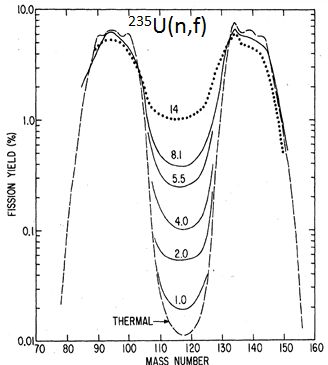
\includegraphics[width=0.9\textwidth]{../figs/FP_Distribution.png}
      \end{figure}
    \end{column}
    
    \begin{column}{0.45\linewidth}
      \vspace{-0.55cm}
      \renewcommand*{\thesubfigure}{}
      \begin{figure}[htp]
        \centering
        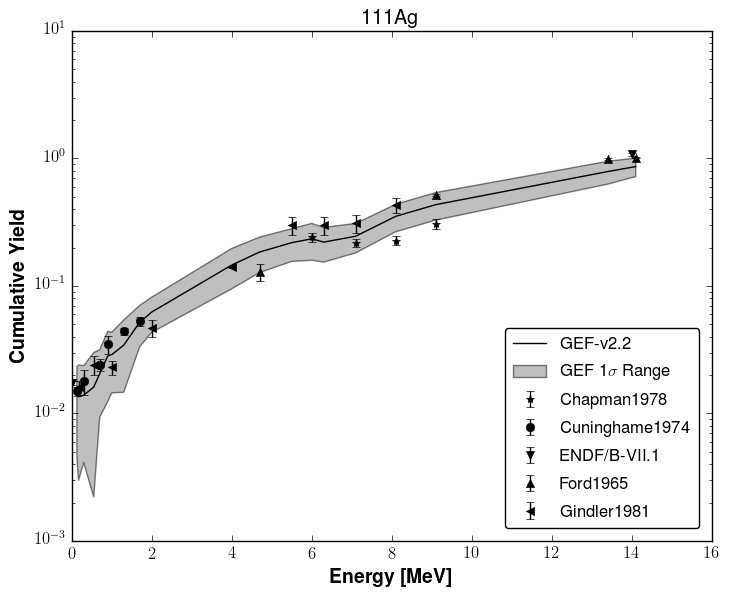
\includegraphics[width=1.45in]{../figs/47_111_Ag_log.png}
        \vspace{-0.35cm}
        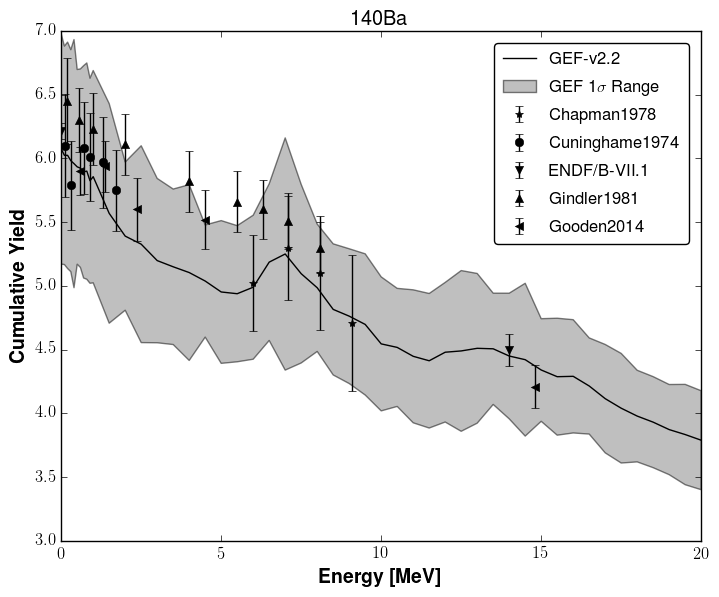
\includegraphics[width=1.45in]{../figs/56_140_Ba_lin.png}
        \vspace{-0.5cm}
        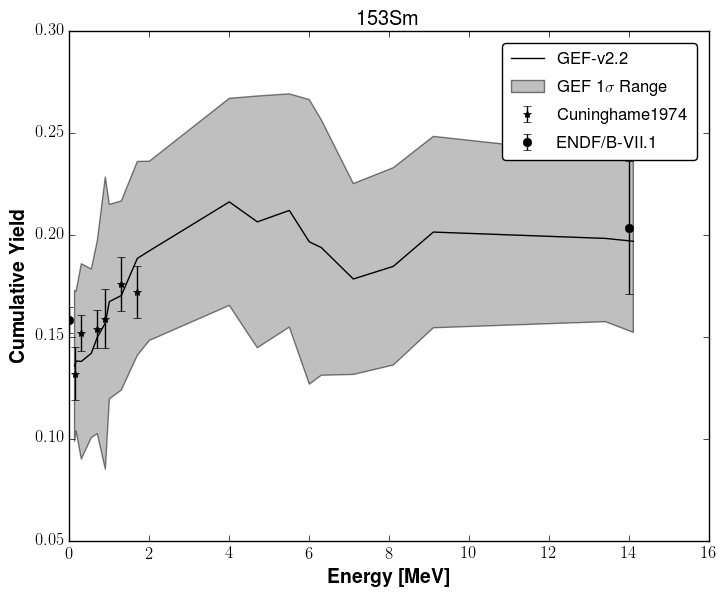
\includegraphics[width=1.45in]{../figs/62_153_Sm_lin.png}
      \end{figure}    
    \end{column}
  \end{columns}   
\end{frame}

% --------------------------------------------------------------
\begin{frame}{Research objectives}
  \centering{\textbf{Develop a capability to design and test custom neutron energy spectra for technical nuclear forensics (TNF)}} 
    \vspace{0.3cm}
    \begin{enumerate}
      \item Design energy tuning assembly (ETA) to generate TNF relevant spectrum at NIF
      \item Piece-wise application specific validation of ETA design at LBNL 88-Inch Cyclotron
      \item Integral test and creation of synthetic debris at NIF
    \end{enumerate}
  \vspace*{-1.5em}
  \renewcommand*{\thesubfigure}{}
  \begin{figure}[htp]
    \centering
    \subcapcentertrue
    \vspace{0.3cm}
    \hspace{0.0cm}
    \subfigure[]{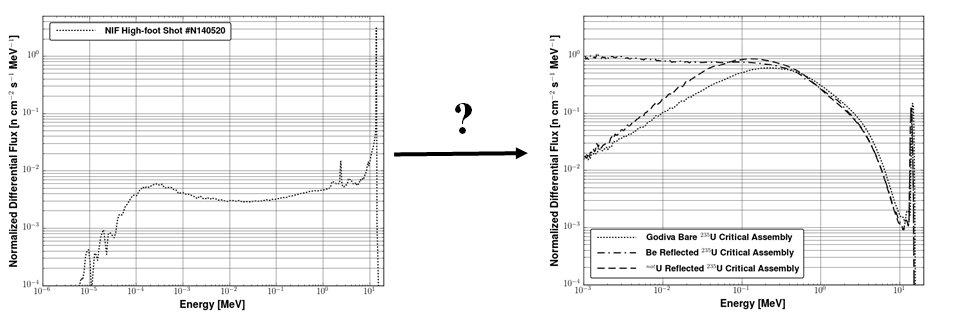
\includegraphics[width=4.5in]{../figs/howto.png}}
  \end{figure}
\end{frame}

% --------------------------------------------------------------
\begin{frame}{Potential application areas}
  \begin{columns}
    \begin{column}{0.5\linewidth}
      \begin{itemize}
        \item Radiation shielding
        \item Radiation effects/damage
        \item Medical physics
        \item Radio-isotope production
      \end{itemize}
      \renewcommand*{\thesubfigure}{}
      \vspace{-0.5cm}
      \begin{figure}[htp]
        \centering
        \subcapcentertrue
        \subfigure{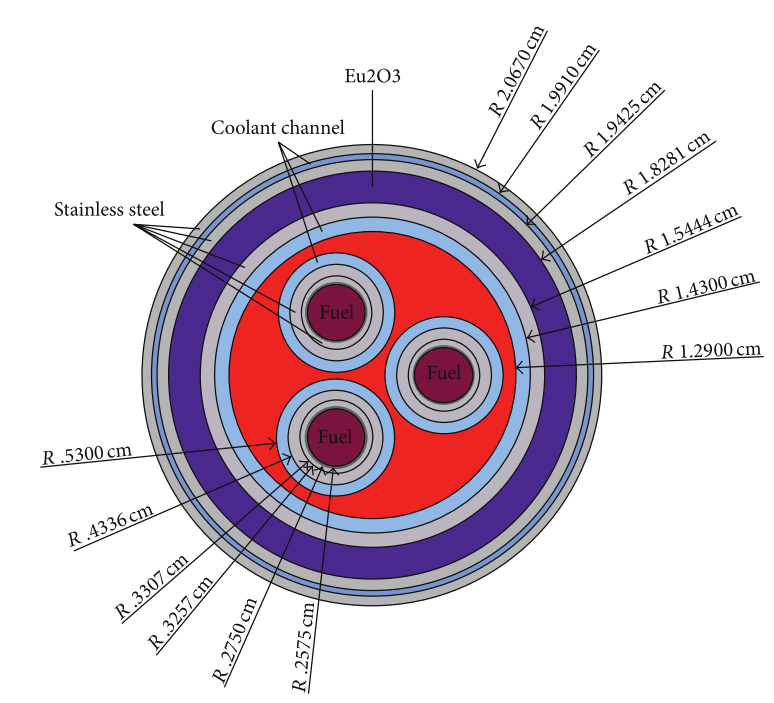
\includegraphics[width=0.85\textwidth]{../figs/HFIR_screen.png}}
      \end{figure}
    \end{column}
    
    \begin{column}{0.5\linewidth}
      \begin{itemize}
        \item Nuclear data
        \item Detector calibration and development
        \item Fusion blanket design
        \item Reactor design
      \end{itemize}
      \renewcommand*{\thesubfigure}{}
      \vspace{-0.5cm}
      \begin{figure}[htp]
        \centering
        \subcapcentertrue
        \subfigure{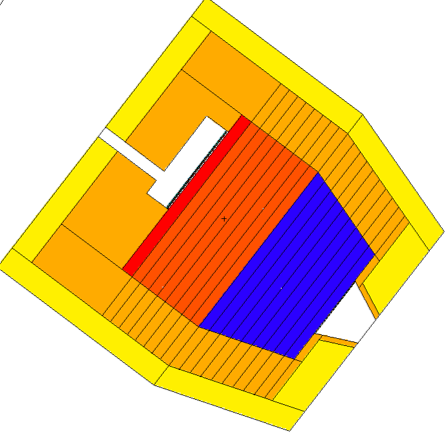
\includegraphics[width=0.75\textwidth]{../figs/BSA.png}}
      \end{figure}
    \end{column}
    
  \end{columns}
\end{frame}

% --------------------------------------------------------------
\begin{frame}{Optimization problem classes}
    Optimization problems can be formulated as \cite{Rady, Yang2014}:
    \begin{myalign}
      &\substack{\text{Minimize}\\\vv{x} \in \mathbb{R}^d}& f_i&(\vv{x}), & (i&=1,\ 2,\ \ldots,\ I) \label{eq:Obj_Funct} \\
      &\text{Subject to:} & h_j&(\vv{x})= 0, & (j&=1,\ 2,\ \ldots,\ J) \label{eq:Eq_Const}\\
      & & g_k&(\vv{x})\le 0, & (k&=1,\ 2,\ \ldots,\ K) \label{eq:Ineq_Const}
    \end{myalign}

    \vspace{-0.15cm}
    where $\vv{x}$ is a vector of the problem design variables     
    
    \vspace{0.25cm}
    Optimization problems can be classified by \cite{Guler2010,Yang2010}:
    \begin{itemize}
      \item Single or multi-objective
      \item Linear or non-linear
      \item Constrained or unconstrained
      \item Continuous or combinatorial (discrete) 
      \item Uni-modal or multi-modal
    \end{itemize}

    \vspace{0.15cm}
    \begin{beamercolorbox}[sep=0pt,rounded=true]{title}
      \usebeamerfont{normal text}\centering%
      \textbf{ETA design is a single objective, non-linear, constrained, continuous \underline{and} discrete multi-modal optimization problem}
    \end{beamercolorbox}    
    
\end{frame}

% --------------------------------------------------------------
\begin{frame}{ETA optimization}
  For the ETA optimization problem, \eqref{eq:Obj_Funct} and \eqref{eq:Ineq_Const} are given by \cite{Chen2010a}: 
  \begin{myalign}
    f_1(\vv{x_p}) &=  \sum_{g=1}^G \left(\frac{\phi^O_g-\phi^D_g(\vv{x_p})}{\phi^O_g}\right)^2 *\frac{\phi^O_g}{\phi^O} \label{eq:ETA_Obj_Funct} \\
    g_1(\vv{x_p}) &=  \displaystyle\sum_{n=1}^{N} \rho_n V_n -W \le 0 \label{eq:ETA_Ineq_Const_1} \\
    g_2(\vv{x_p}) &=  N_f^{min} - n \phi V(\sigma^{235}_f+\sigma^{238}_f) \le 0 \label{eq:ETA_Ineq_Const_2}
  \end{myalign}
  
  Where $\phi^O$ is the design objective neutron spectrum and $\phi^D(\vv{x_p})$ is the neutron spectra corresponding to a candidate design \newline
  
  $\vv{x_p}$ is a vector of the variables for a candidate design given by (in 2-D):
  \begin{myalign}
    \begin{split}     
      \vv{x_p}=\{&Cell_1[M_1, \rho_1, IR_1, OR_1, Z1_1, Z2_1],\  Cell_2[\ldots],\  \dots, \\
      &Cell_N[M_N, \rho_N, IR_N, OR_N, Z1_N, Z2_N],\ R_{foil},\ Z_{foil}\}
    \end{split}
  \end{myalign}
  
%  \begin{equation}
%    P=(|M| \times |\rho| \times |IR| \times |OR| \times |Z1| \times |Z2|)^{|N|} \times |R_{foil}| \times |Z_{foil}|
%  \end{equation} 
\end{frame}

% --------------------------------------------------------------
\begin{frame}{Optimization methods: metaheuristics \cite{Lones2014}}
  \vspace{-0.25cm}
  \renewcommand*{\thesubfigure}{}
  \begin{figure}[htp]
    \centering
    %\captionsetup{justification=centering,margin=0cm}
    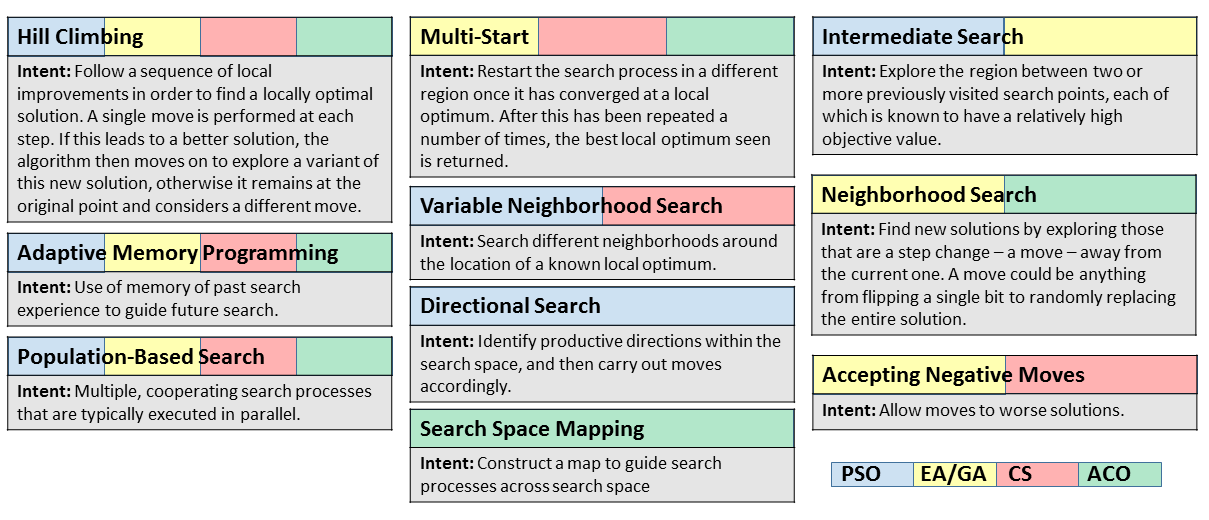
\includegraphics[width=1.1\textwidth]{../figs/Heuristics.png}
  \end{figure}
\end{frame}

% --------------------------------------------------------------
\begin{frame}{
\includegraphics[width=0.35in]{../figs/Gnowee.png} \hspace{0.25cm}  Gnowee: hybrid metaheuristic opt.}
  \centering{\textbf{\underline{General purpose} metaheuristic optimization algorithm }}
  \begin{columns}
    \begin{column}{0.6\linewidth}
      \vspace{-0.75cm}
      \begin{itemize}
        \item Handles continuous and discrete variables \newline
        \item Robust, complete set of search heuristics \newline
        \item Nearly-global convergence \newline
        \item Outperforms most other algorithms we tested on all nearly all problems of interest
      \end{itemize} 
    \end{column}
    
    \begin{column}{0.4\linewidth}
      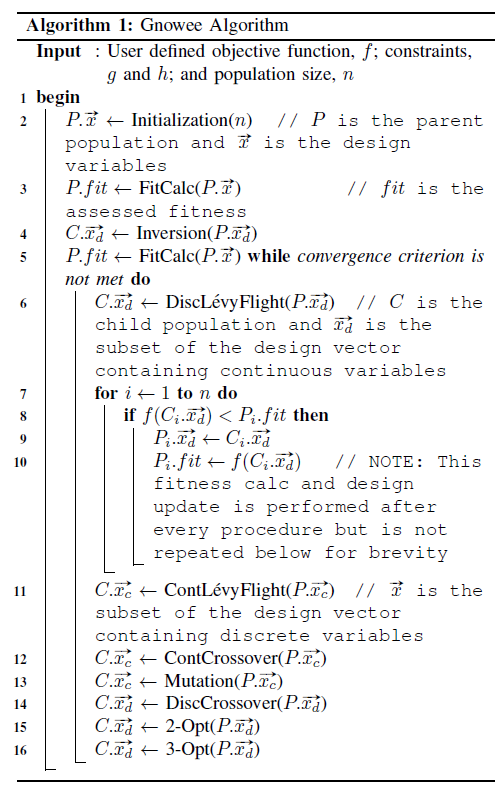
\includegraphics[width=0.95\textwidth]{../figs/GnoweeAlgorithm.png}
    \end{column}
  \end{columns}
\end{frame}

% --------------------------------------------------------------
\begin{frame}{
\includegraphics[width=0.35in]{../figs/Gnowee.png} Gnowee: Benchmarking \cite{Walton2013a,Yang2014,Civicioglu2013}}
  \begin{columns}
    \begin{column}{0.33\linewidth} 
      \vspace{-.5cm} 
      \begin{figure}[htp]
        \centering
        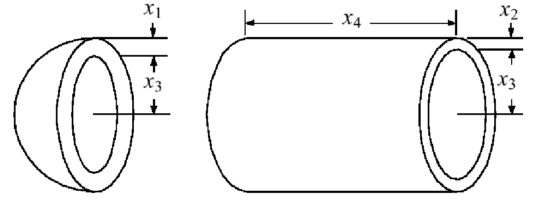
\includegraphics[width=1.0\textwidth, height=0.18\textheight]{../figs/PressureVessel.png} 
      \end{figure}        
      \vspace{-0.75cm} 
      \begin{figure}[htp]
        \centering
        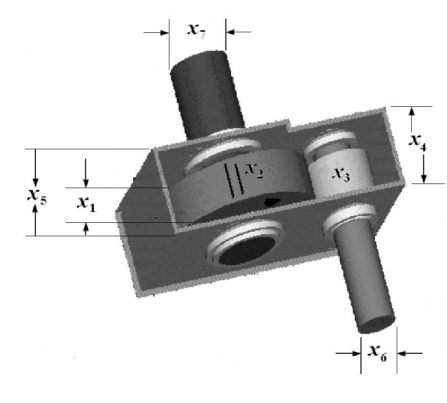
\includegraphics[width=1.0\textwidth, height=0.27\textheight]{../figs/SpeedReducer.png} 
      \end{figure}       
      \vspace{-0.75cm} 
%      \begin{figure}[htp]
%        \centering
%        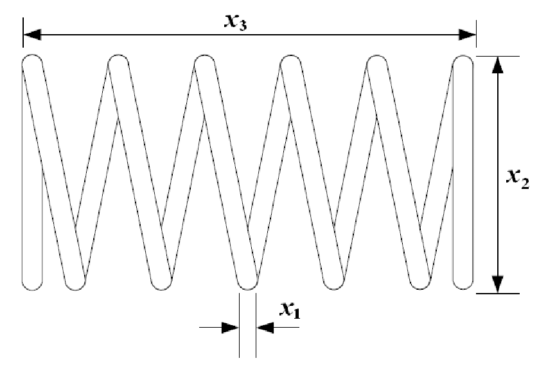
\includegraphics[width=1.0\textwidth, height=0.18\textheight]{../figs/Spring.png} 
%      \end{figure}       
%      \vspace{-0.750cm} 
      \begin{figure}[htp]
        \centering
        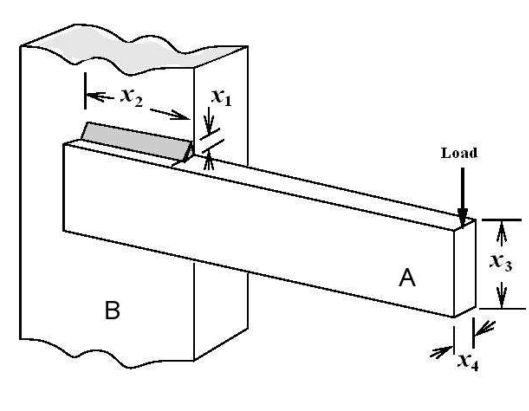
\includegraphics[width=1.0\textwidth, height=0.20\textheight]{../figs/WeldedBeam.png} 
      \end{figure}
    \end{column}
    
    \begin{column}{0.33\linewidth}
      \vspace{-.55cm} 
      \begin{figure}[htp]
        \centering
        %\captionsetup{justification=centering,margin=0cm,labelformat=empty}
        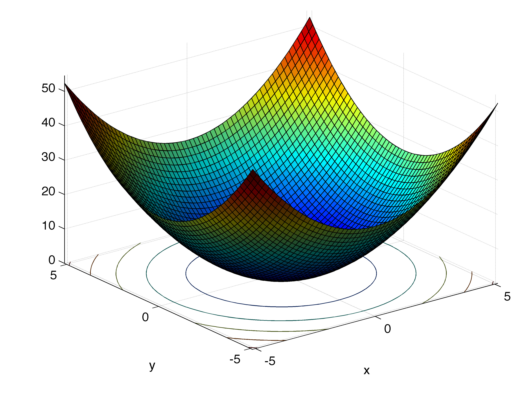
\includegraphics[width=1.0\textwidth, height=0.25\textheight]{../figs/DeJong.png} 
        \vspace{-0.35cm}
        %\caption*{De Jong}
      \end{figure}        
      \vspace{-1.05cm} 
      \begin{figure}[htp]
        \centering
        %\captionsetup{justification=centering,margin=0cm}
        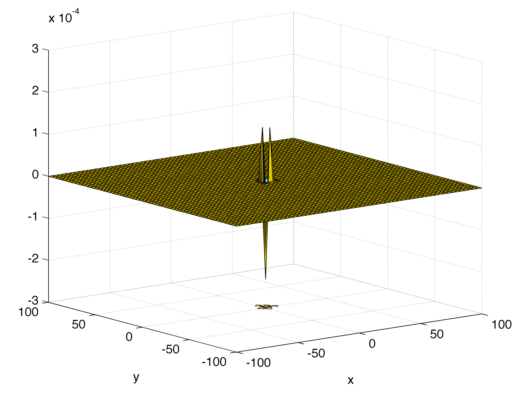
\includegraphics[width=1.0\textwidth, height=0.25\textheight]{../figs/Easom.png} 
        \vspace{-0.35cm}
        %\caption*{ Easom}
      \end{figure}       
      \vspace{-1.05cm} 
      \begin{figure}[htp]
        \centering
        %\captionsetup{justification=centering,margin=0cm}
        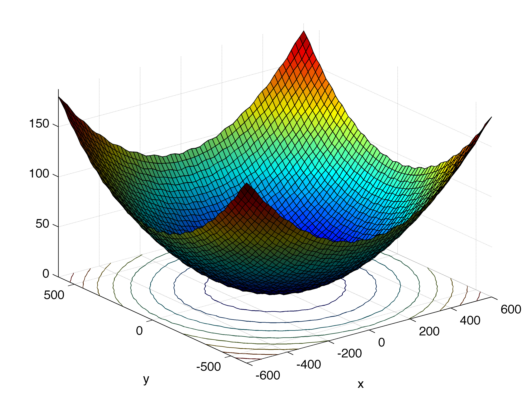
\includegraphics[width=1.0\textwidth, height=0.25\textheight]{../figs/Griewank.png} 
        \vspace{-0.35cm}
        %\caption*{Griewank}
      \end{figure}
    \end{column}
    
    \begin{column}{0.33\linewidth}
      \vspace{-.9cm} 
      \begin{figure}[htp]
        \centering
        %\captionsetup{justification=centering,margin=0cm}
        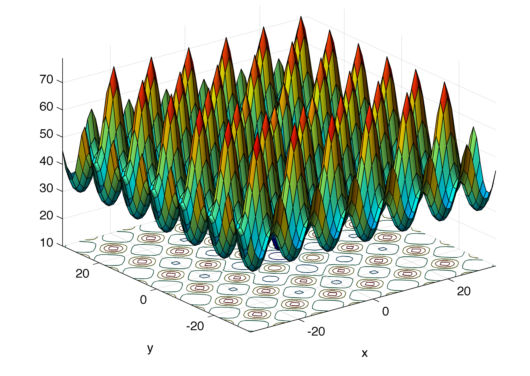
\includegraphics[width=1.0\textwidth, height=0.25\textheight]{../figs/Ackley.png} 
        \vspace{-0.35cm}
        %\caption*{Ackley}
      \end{figure}        
      \vspace{-1.4cm} 
      \begin{figure}[htp]
        \centering
        %\captionsetup{justification=centering,margin=0cm}
        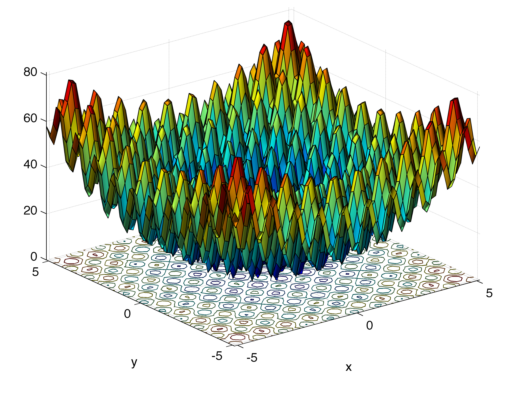
\includegraphics[width=1.0\textwidth, height=0.25\textheight]{../figs/Rastrigin.png} 
        \vspace{-0.35cm}
        %\caption*{Rastrigin}
      \end{figure}       
      \vspace{-1.15cm} 
      \begin{figure}[htp]
        \centering
        %\captionsetup{justification=centering,margin=0cm}
        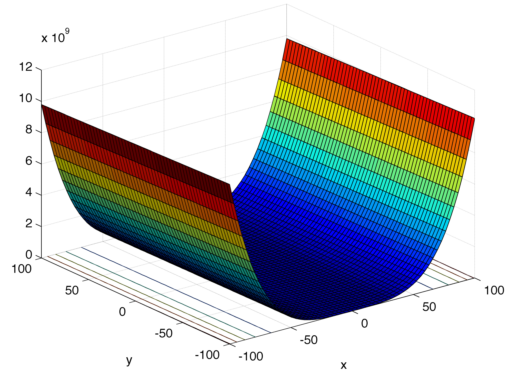
\includegraphics[width=1.0\textwidth, height=0.25\textheight]{../figs/Rosenbrock.png} 
        \vspace{-0.35cm}
        %S\caption*{Rosenbrock}
      \end{figure}
    \end{column}
  \end{columns}
\end{frame}

% --------------------------------------------------------------
\begin{frame}{
\includegraphics[width=0.35in]{../figs/Coeus.jpg}  \hspace{0.25cm}  Coeus: NE optimization software}
  \centering{\textbf{ETA design tool to build custom neutron spectra from existing facilities and sources}}
  
  \begin{itemize}
    \item MCNP-Denovo hybrid radiation transport engine \cite{MCNP2008, ORNL2015, Evans2010}
    \item ETA designs generated with Gnowee optimization framework 
    \item Fully operational on Savio -- neutronics design in days
    \item Expanding capabilities by adding more objective functions, constraints, and geometric options     
  \end{itemize}
  
%  \begin{columns}
%  \begin{column}{0.5\linewidth}
%    \centering
%    \subcapcentertrue
%    \vspace{-0.2cm}  
%      \centering
%      \begin{animateinline}[autoplay,loop]{2}  
%      \multiframe{33}{i=0+1}{%
%      \includegraphics[width=0.65\textwidth]{gifs/ETA_\i.png}}
%      \newframe
%      \includegraphics[width=0.65\textwidth]{gifs/ETA_32.png}
%      \newframe[1]
%      \includegraphics[width=0.65\textwidth]{gifs/ETA_32.png}
%  \end{animateinline} 
%  \end{column}
%  
%  \begin{column}{0.6\linewidth}
%    %\vspace{-1.25cm}
%    \includemedia[
%      activate=pageopen,
%      width=0.75\textwidth,height=0.44\textheight,
%      addresource=figs/results.mp4,
%      flashvars={%
%        source=figs/results.mp4
%        &autoPlay=true%    % optional configuration
%        &loop=true%        % variables
%        }  
%    ]{}{VPlayer9.swf}
%  \end{column}
%  \end{columns}
\end{frame}

% --------------------------------------------------------------
\begin{frame}{Development Approach}
  \begin{columns}
    \begin{column}{0.55\linewidth}
      \begin{itemize}
        \item 1.2 g HEU foil
        \item $\sim80$ kg
        \item \SI{1e+8} - \SI{1e+9} Fissions
      \end{itemize}  
      
      \renewcommand*{\thesubfigure}{}
      \begin{figure}[htp]
        \centering
        \subcapcentertrue
        \vspace{-0.6cm}
        \subfigure[\small ETA Design]{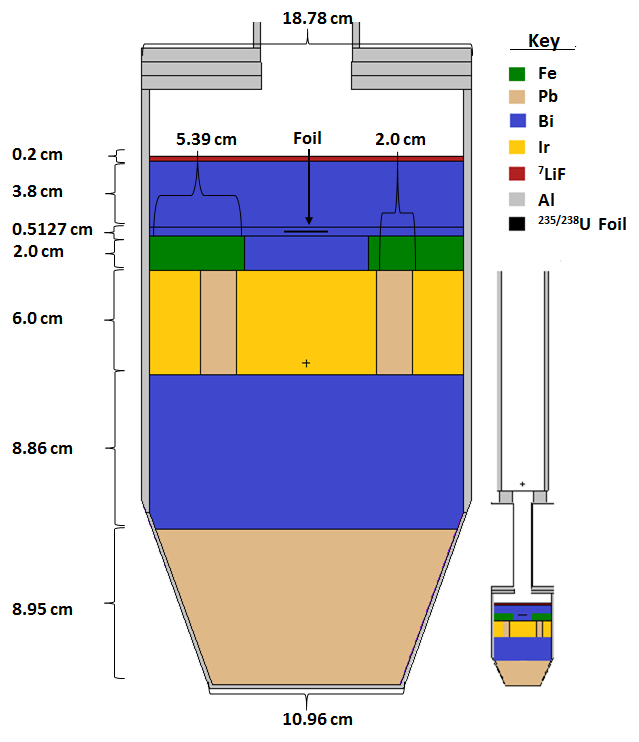
\includegraphics[width=1.9in]{../figs/ETA_Design_1g235.png}}
      \end{figure}
    \end{column}
    
    \begin{column}{0.5\linewidth}
      \vspace{-1cm}      
      \renewcommand*{\thesubfigure}{}
      \begin{figure}[htp]
        \centering
        \subcapcentertrue
        \subfigure[]{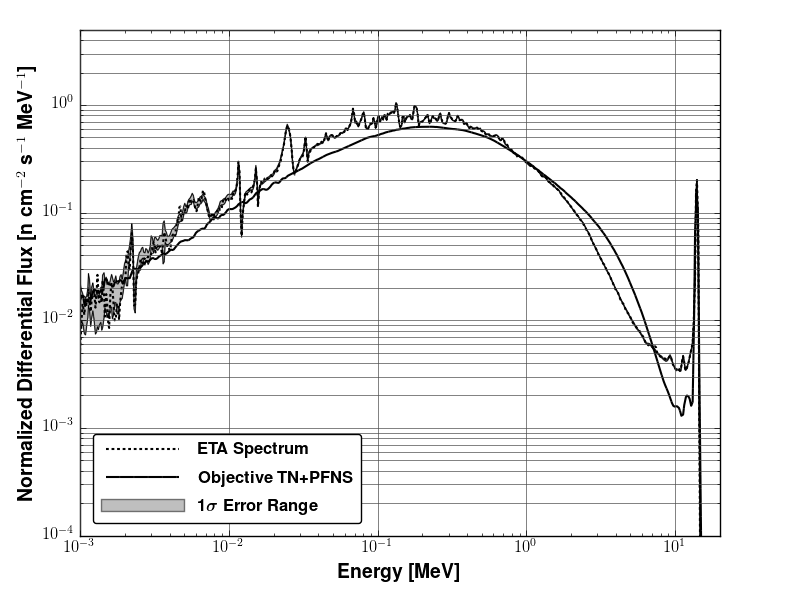
\includegraphics[width=2.2in]{../figs/ETA_Output_vs_Obj_1g.png}}
      \end{figure}
      
      \vspace{-1.4cm}
      \begin{table}
        \centering
        \tiny
        \begin{tabular}{0.95\textwidth}%{@{} Y c c @{}} 
          \toprule
          \textbf{Energy} & \textbf{Target Normalized} & \textbf{\% Fluence} \\
          \textbf{Range} & \textbf{Differential Fluence} & \textbf{Achieved} \\
          \midrule
          0-3 keV & \SI{6.24e-05} & 103.4 $\mypm$ 2.0\% \\ \addlinespace
          3-100 keV & \SI{3.41e-02} & 140.7 $\mypm$ 0.1\% \\ \addlinespace
          0.1-6 MeV & \SI{8.46e-01} & 96.0 $\mypm$ 0.0\% \\ \addlinespace
          6-10 MeV & \SI{1.65E-02} & 117.3 $\mypm$ 0.2\% \\ \addlinespace
          10-16 MeV & \SI{1.01E-01} & 119.4 $\mypm$ 0.0\% \\ \addlinespace
          \bottomrule
        \end{tabular} 
      \end{table}
      \vspace{-0.2cm}      
      \small \centering ETA vs Objective Spectrum 
    \end{column}
  \end{columns}    
\end{frame}

% --------------------------------------------------------------
\begin{frame}{NIF experiment: TNF validation}
    \textbf{Experimental Overview:}
    \begin{itemize}
      \item $\sim$\SI{1.0e+15} neutrons in 4$\pi$
      \item Minimize $\rho$R in direction of the ETA DIM 
      \item ETA fielded as snout on DIM DLP located 75 mm from TCC
          
        \vspace{-0.25cm}
  \renewcommand*{\thesubfigure}{}
  \begin{figure}[htp]
    \centering
    \subcapcentertrue
    \subfigure[]{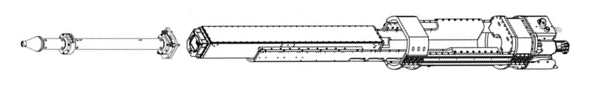
\includegraphics[width=3.25in]{../figs/DIM_schematic.png}}
  \end{figure} 
  
        \vspace{-1.0cm}  
      \item No on-line DIM diagnostics required
      \item Radio-chemistry and gamma spectroscopy facilities required post-shot
      \item NTOF, FNADS, and MRS required to measure the source term 
    \end{itemize}
    
\end{frame}

% --------------------------------------------------------------
\begin{frame}{NIF experiment: TNF validation}

    \textbf{Expected Experimental Outcomes:}
      \begin{columns}
        \begin{column}{0.5\linewidth}
          \vspace{-0.15	cm} 
          \begin{itemize}
            \item Generation of realistic FP distribution
            \item Quantification of spectrum through fission splits
            \item Unfolding of spectrum using activation analysis
          \end{itemize}
        \end{column}
        
        \begin{column}{0.5\linewidth}
          \includegraphics[width=2.0in]{../figs/NAS2.png}
        \end{column}
      \end{columns}
\end{frame}

% --------------------------------------------------------------
\begin{frame}{88-Inch experiments: TNF validation}
      \begin{columns}
        \begin{column}{0.55\linewidth}
          \begin{itemize}
            \item 29/33 MeV D-breakup on Ta
            \item Field NIF ETA design
            \item Field partial ETA stackups
            \item EJ-309 detectors, activation, and fission products measurements 
          \end{itemize}
          \includegraphics[width=0.95\textwidth]{../figs/33MeVTa_OutputComp.png}
        \end{column}
        
        \begin{column}{0.45\linewidth}
          \includegraphics[width=0.75\textwidth]{../figs/88InchLayout.png}
        \end{column}
      \end{columns}
\end{frame}

% --------------------------------------------------------------
\begin{frame}{Project 2 Summary}
  \begin{itemize}
    \item Spectral shaping methods can be used to expand the capabilities of existing facilities to cover new mission spaces \newline
    \item Coeus provides an efficient capability to design and optimize ETAs for spectral shaping 
    \begin{itemize}
      \item \textit{\underline{Not}} input or output specific
      \item Further development to improve user flexibility underway \newline
    \end{itemize}
    \item Experimental validation of TNF application at LBNL 88-Inch Cyclotron executed \newline
    \item Planning underway for NIF shot
    \begin{itemize}
      \item Scoping study has shown feasibility
      \item Partial funding/support from DNDO/NTNFC, DTRA, and LANL \newline
    \end{itemize}
      
  \end{itemize}
\end{frame}

% --------------------------------------------------------------
% --------------------------------------------------------------
\section*{}
\begin{frame}[fragile]
  %\frametitle{Questions?}
        \begin{columns}
        \begin{column}{0.55\linewidth}
          \includegraphics[width=0.95\textwidth]{../figs/earth}
        \end{column}
        
        \begin{column}{0.45\linewidth}
We would accomplish many more things if we did not think of them as impossible. \\
\vspace*{1em}
- Vince Lombardi
        \end{column}
      \end{columns}
  \begin{center}
  \end{center}
  
\end{frame}

% --------------------------------------------------------------
\begin{frame}{Summary}
  \begin{itemize}
    \item Innovation is needed for many nuclear technologies \newline
    \item Predictive simulation can play a key role \newline
    \item We're developing better hybrid methods 
    \begin{itemize}
      \item for problems with strong anisotropies
      \item and to provide evaluative flexibility \newline
    \end{itemize}
    \item Energy tuning assemblies can provide strategic investigative tools
    \begin{itemize}
      \item for technical nuclear forensics
      \item as well as many other applications
    \end{itemize}
      
  \end{itemize}
\end{frame}

% --------------------------------------------------------------
% --------------------------------------------------------------
\section*{}
\begin{frame}[fragile]
  \frametitle{Questions?}
  \begin{center}
  \includegraphics[height=3in,clip]{../questions-comic}  
  \end{center}
  
\end{frame}

% --------------------------------------------------------------
\begin{frame}{Acknowledgments }
 	  \footnotesize{\textbf{University of California, Berkeley:}
	  \begin{itemize}
	    \item Madicken Munk, Kelly Rowland, Richard Vasques
	    \item James Bevins, Bethany Goldblum, Josh Brown, Matthew Harasty, Will Kable, Ethan Boado, Sandra Bogetic, Youdong Zhang
	  \end{itemize}
	  
	  \textbf{Oak Ridge National Lab:}
	    \begin{itemize}
	      \item Tom Evans, Steven Hamilton, Scott Mosher, Tara Pandya, Seth Johnson, Josh Jarrell
	    \end{itemize}
	    
	  \textbf{Lawrence Berkeley National Lab:}
	    \begin{itemize}
	      \item Lee Bernstein
	    \end{itemize}
	    
	  \textbf{Lawrence Livermore National Lab:}
	  \begin{itemize}
	    \item Bill Dunlop, Eugene Henry, Darren Bleuel, Brent Blue, Walid Younes, Joe Bauer, Dawn Shaughnessy, Narek Gharibyan, Don Jedlovec, Charles Yeamans, Kim Christensen 
	  \end{itemize}}
\end{frame}

% --------------------------------------------------------------
\begin{frame}{Disclaimers}
\centering  
The views expressed in this research are those of the author and do not reflect the official policy or position of the United States Air Force, the Department of Defense, or the United States Government. \newline
\vspace{0.5cm}  

This material is based upon work supported by the National Science Foundation Graduate Research Fellowship Program and Department of Energy award number DE-NE0008286. Any opinions, findings, and conclusions or recommendations expressed in this material are those of the author(s) and do not necessarily reflect the views of the National Science Foundation.
\end{frame}


% --------------------------------------------------------------
\begin{frame}[plain,allowframebreaks]{References}
\small
        \bibliographystyle{unsrt}
	\bibliography{2017-05-lbnl}%\printbibliography
\end{frame}

%\begin{frame}[allowframebreaks]{References}
%	\bibliographystyle{unsrt}
%	\bibliography{2017-03-mpact}
%\end{frame}

\end{document}
